\documentclass{article}
% \usepackage{txfonts}
% \usepackage{graphicx}
%导言区
\usepackage{graphicx}
\usepackage{epstopdf}
\usepackage{float} 
\usepackage{subfigure}
\usepackage[]{caption2}
\begin{document}

2.2.1 $ \dot x =4x^2-16 $

\begin{figure}[H]
\centering
\subfigure[2.2.1]{
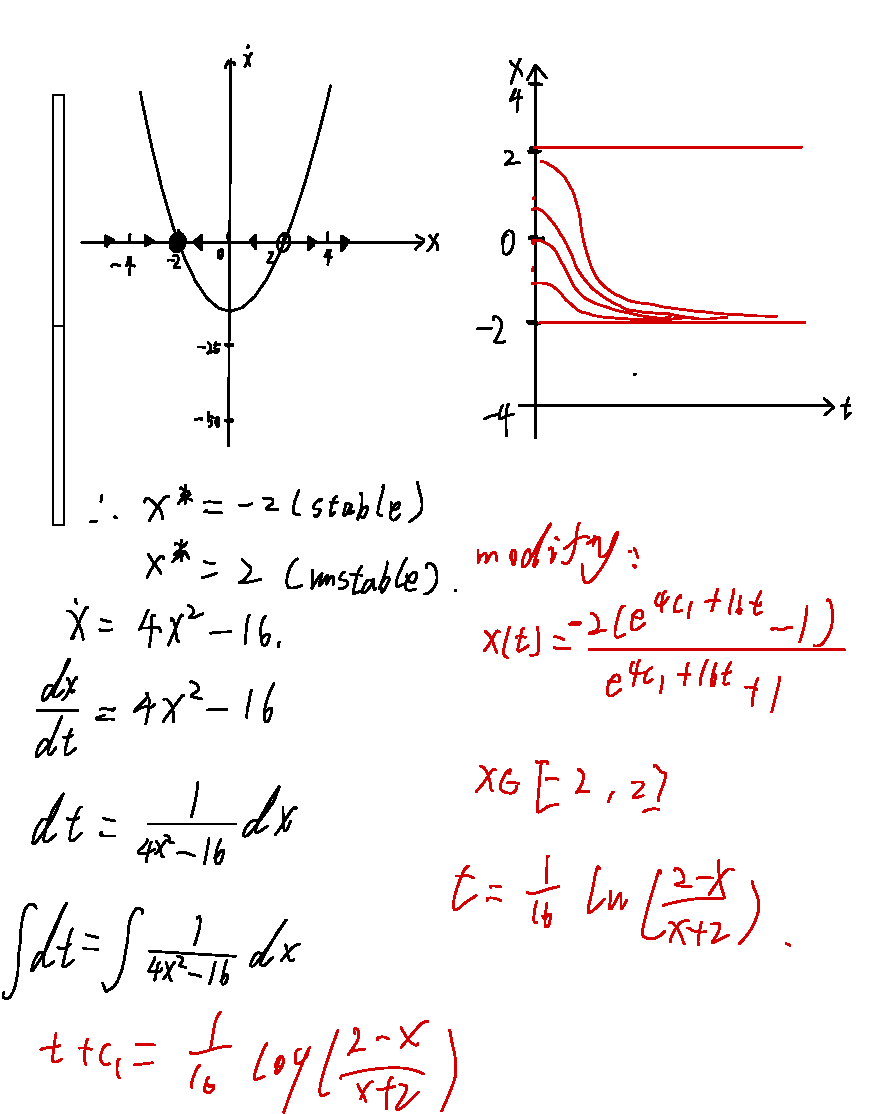
\includegraphics[scale=0.7]{/Users/soliva/Desktop/Homework/Nonlinear_Dynamics/latexfile/m221.pdf}}
\end{figure}

2.2.8

\begin{figure}[H]
\centering
\subfigure[2.2.8]{
\includegraphics[scale=0.7]{/Users/soliva/Desktop/Homework/Nonlinear_Dynamics/latexfile/m228.pdf}}
\end{figure}
2.4.3 

\begin{figure}[H]
\centering
\subfigure[2.4.3]{
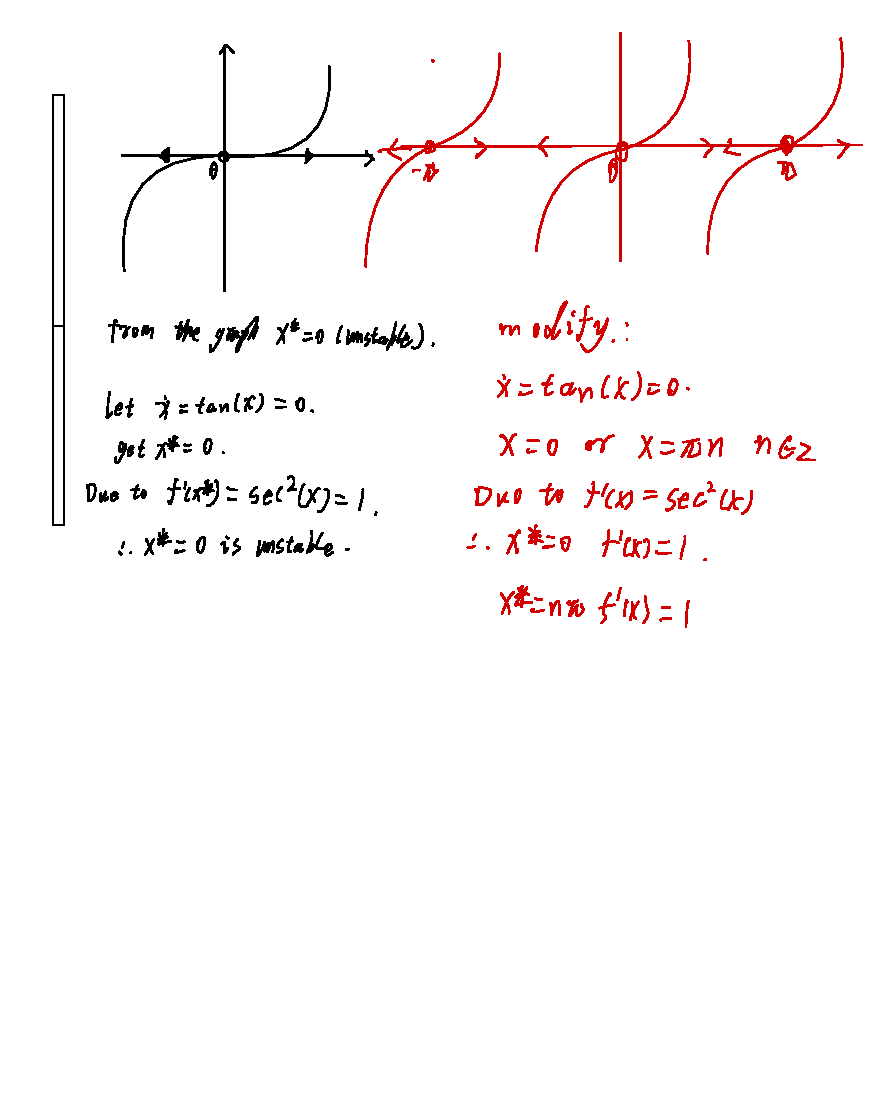
\includegraphics[scale=0.7]{/Users/soliva/Desktop/Homework/Nonlinear_Dynamics/latexfile/m243.pdf}}
\end{figure}

3.2.3
\begin{figure}[H]
\centering
\subfigure[3.2.3]{
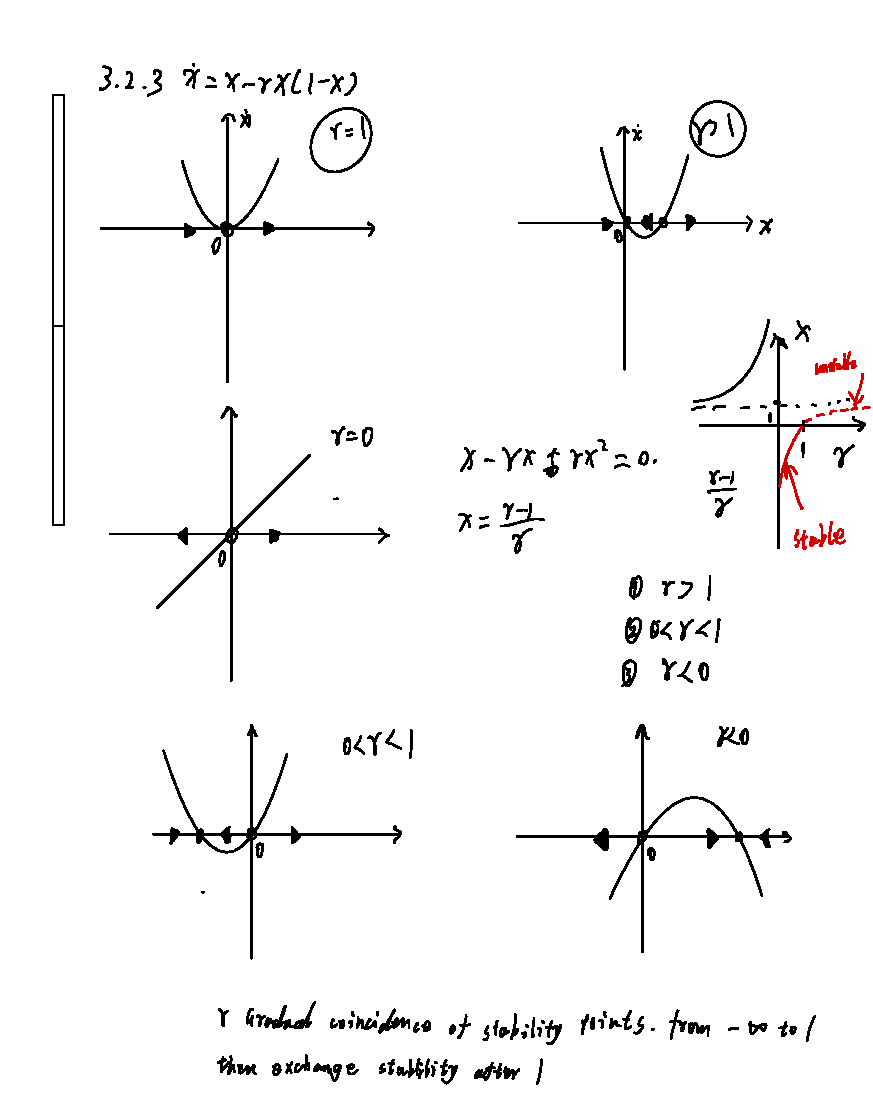
\includegraphics[scale=0.7]{/Users/soliva/Desktop/Homework/Nonlinear_Dynamics/latexfile/m323.pdf}}
\end{figure}


3.4.6
\begin{figure}[H]
\centering
\subfigure[3.4.6]{
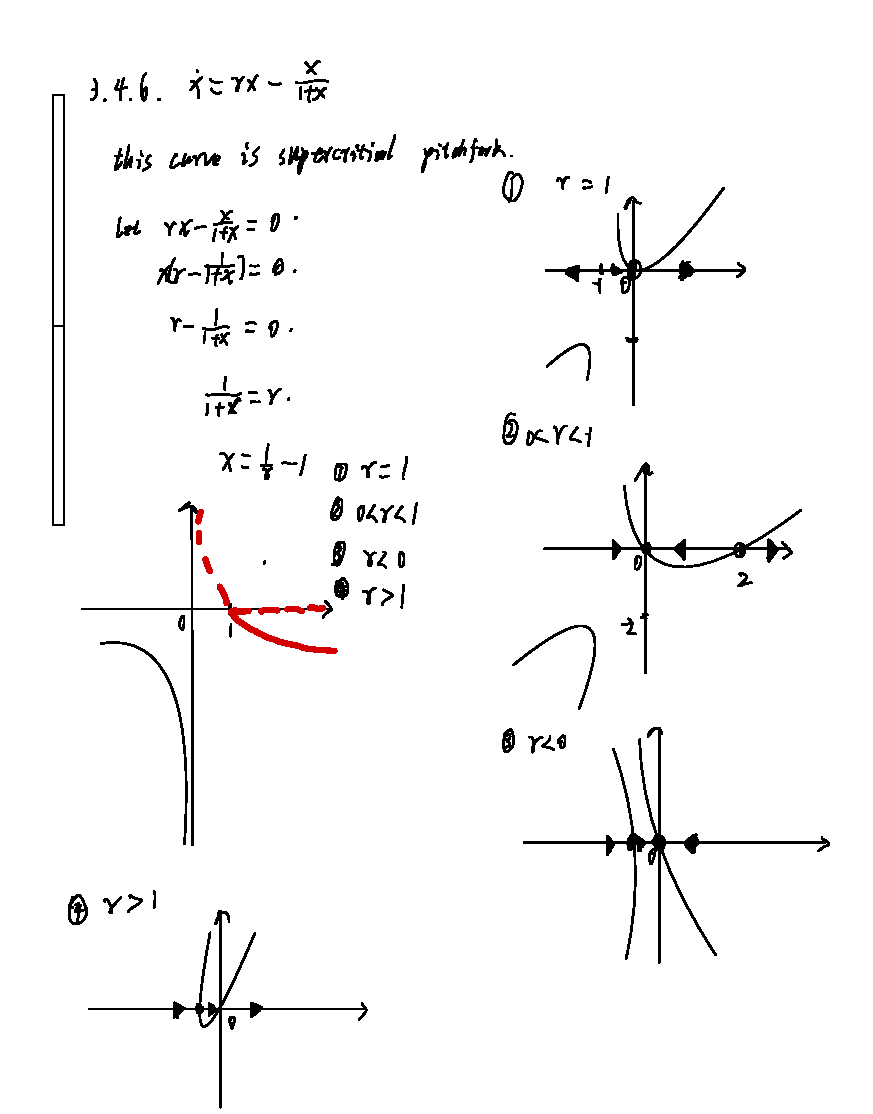
\includegraphics[scale=0.7]{/Users/soliva/Desktop/Homework/Nonlinear_Dynamics/latexfile/m346.pdf}}
\end{figure}


5.1.7
\begin{figure}[H]
\centering
\subfigure[5.1.7]{
\includegraphics[scale=0.7]{/Users/soliva/Desktop/Homework/Nonlinear_Dynamics/latexfile/m517.pdf}}
\end{figure}


5.2.3
\begin{figure}[H]
\centering
\subfigure[5.2.3]{
\includegraphics[scale=0.7]{/Users/soliva/Desktop/Homework/Nonlinear_Dynamics/latexfile/m523.pdf}}
\end{figure}

5.2.5
\begin{figure}[H]
\centering
\subfigure[5.2.5]{
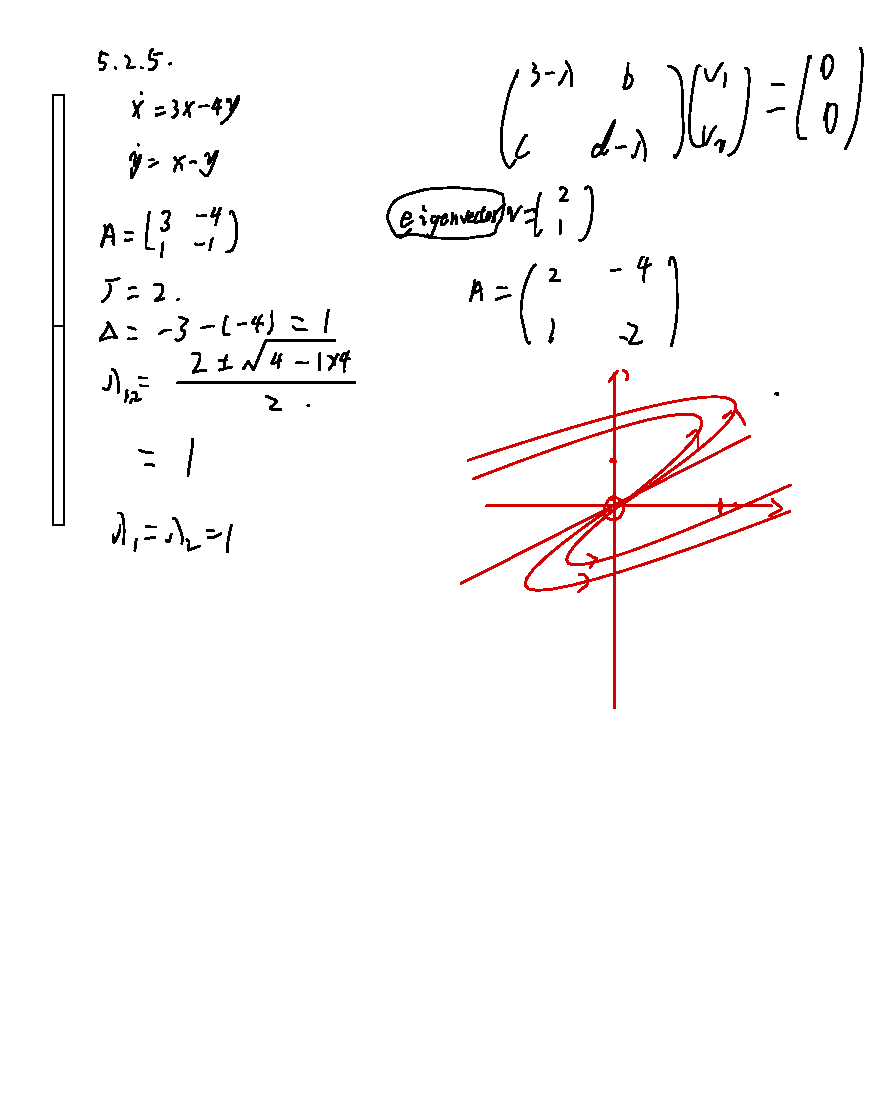
\includegraphics[scale=0.7]{/Users/soliva/Desktop/Homework/Nonlinear_Dynamics/latexfile/m525.pdf}}
\end{figure}


5.3.4

\begin{figure}[H]
\centering
\subfigure[5.3.4]{
\includegraphics[scale=0.7]{/Users/soliva/Desktop/Homework/Nonlinear_Dynamics/latexfile/m534.pdf}}
\end{figure}
6.3.1
\begin{figure}[H]
          \centering
          \subfigure[6.3.1]{
          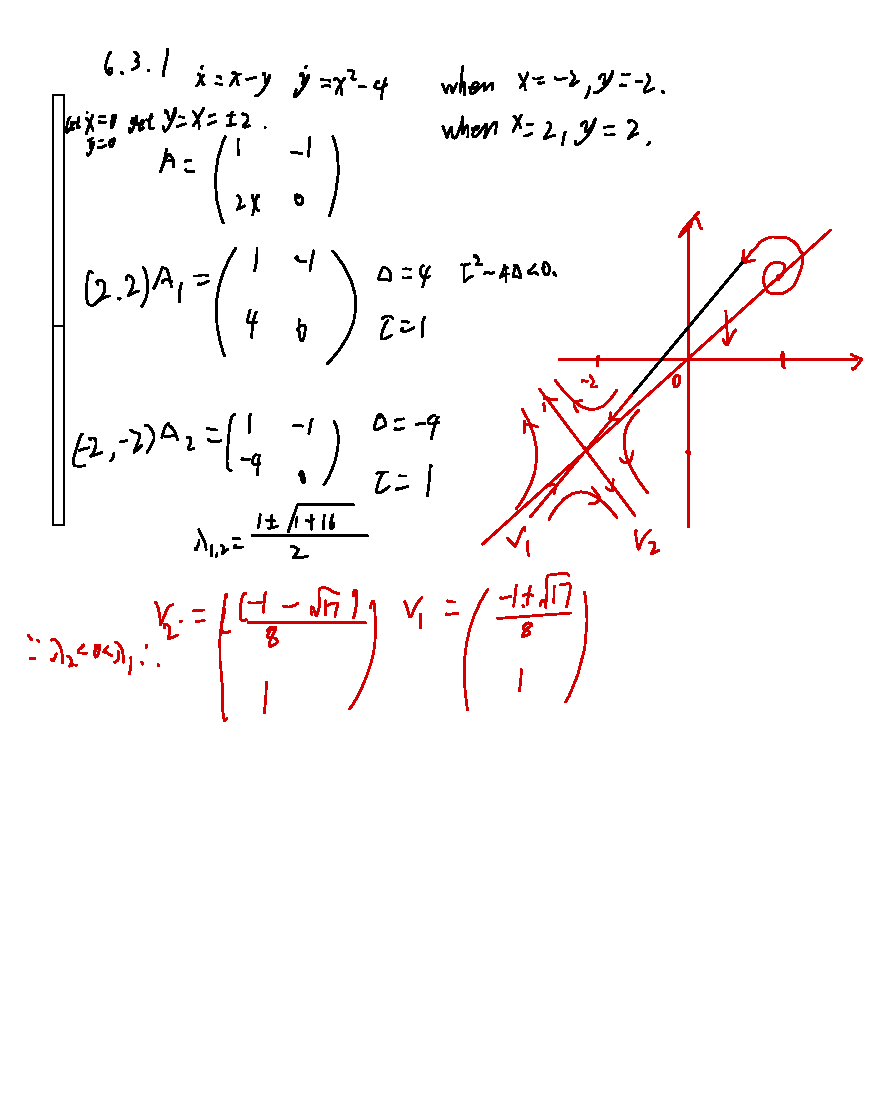
\includegraphics[scale=0.7]{/Users/soliva/Desktop/Homework/Nonlinear_Dynamics/latexfile/m631.pdf}}
          \end{figure}
6.3.3
\begin{figure}[H]
\centering
\subfigure[6.3.3]{
\includegraphics[scale=0.7]{/Users/soliva/Desktop/Homework/Nonlinear_Dynamics/latexfile/633.pdf}}
\end{figure}


6.4.2
\begin{figure}[H]
\centering
\subfigure[6.4.2]{
\includegraphics[scale=0.7]{/Users/soliva/Desktop/Homework/Nonlinear_Dynamics/latexfile/m642.pdf}}
\end{figure}


\end{document}